
\documentclass[10pt]{article}

\usepackage{amsthm}
\usepackage[toc,page]{appendix}
\usepackage{amssymb}
\usepackage{bm}
\usepackage{pslatex,palatino,avant,graphicx,color}
\usepackage{colortbl}
\usepackage{fullpage}
\usepackage{mathtools}
\usepackage{natbib}
\usepackage{amsmath}
\usepackage{caption}
%\usepackage{subfigure}
\usepackage{subcaption}
\usepackage{bm}
\usepackage{wrapfig}
\usepackage{enumerate}
\usepackage{rotating}
\usepackage{multirow}
\usepackage{tabularx}
\usepackage{tikz}
\usepackage{pgfplots}
\usepackage{bbm}
\usepackage[titles,subfigure]{tocloft} % Alter the style of the Table of Contents

\newtheorem{lemma}{Lemma}
%\pdfminorversion=4
% NOTE: To produce blinded version, replace "0" with "1" below.
\newcommand{\blind}{0}

% DON'T change margins - should be 1 inch all around.
\addtolength{\oddsidemargin}{0in}%
\addtolength{\evensidemargin}{0in}%
\addtolength{\textwidth}{0in}%
\addtolength{\textheight}{0in}%
\addtolength{\topmargin}{0in}%


\renewcommand{\cftsecfont}{\rmfamily\mdseries\upshape}
\renewcommand{\cftsecpagefont}{\rmfamily\mdseries\upshape} % No bold!

\newcommand{\indicator}[1]{\mathbbm{1}\left( #1 \right) }
\newcommand{\hb}{\hat{b}}
\newcommand{\ha}{\hat{a}}
\newcommand{\htheta}{\hat{\theta}}
\newcommand{\halpha}{\hat{\alpha}}
\newcommand{\hmu}{\hat{\mu}}
\newcommand{\hsigma}{\hat{\sigma}}
\newcommand{\hphi}{\hat{\phi}}
\newcommand{\htau}{\hat{\tau}}
\newcommand{\heta}{\hat{\eta}}
\newcommand{\E}[1]{\mbox{E}\left[#1\right]}
\newcommand{\Var}[1]{\mbox{Var}\left[#1\right]}
\newcommand{\Indicator}[1]{\mathbbm{1}_{ \left( #1 \right) } }
\newcommand{\dNormal}[3]{ N\left( #1 \left| #2, #3 \right. \right) }
\newcommand{\Beta}[2]{\mbox{Beta}\left( #1, #2 \right)}
\newcommand{\alphaphi}{\alpha_{\hphi}}
\newcommand{\betaphi}{\beta_{\hphi}}
\newcommand{\expo}[1]{ \exp\left\{ #1 \right\}}
\newcommand{\tauSquareDelta}{\htau^2
  \left(\frac{1-\expo{-2\htheta\Delta}}{2\htheta} \right)}
\newcommand{\mumu}{\mu_{\hmu}}
\newcommand{\sigmamu}{\sigma^2_{\hmu}}
\newcommand{\sigmamuexpr}{\log\left( \frac{\VarX}{\EX^2} + 1 \right)}
\newcommand{\mumuexpr}{\log(\EX) -  \log\left( \frac{\VarX}{\EX^2} + 1 \right) /2 }

\newcommand{\EX}{\mbox{E}\left[ X \right] }
\newcommand{\VarX}{\mbox{Var}\left[ X \right] }
\newcommand{\mueta}{\mu_{\heta} }
\newcommand{\sigmaeta}{\sigma^2_{\heta}}
\newcommand{\sigmaetaexpr}{ \log\left( \frac{\VarX}{\EX^2} + 1 \right) }
\newcommand{\muetaexpr}{ \log(\EX) -  \sigmaetaexpr /2 }

\newcommand{\mualpha}{\mu_{\halpha} }
\newcommand{\sigmaalpha}{\sigma^2_{\halpha}}
\newcommand{\sigmaalphaexpr}{ \log\left( \frac{\VarX}{\EX^2} + 1 \right) }
\newcommand{\mualphaexpr}{ \log(\EX) -  \sigmaalphaexpr /2 }

\newcommand{\mutauexpr}{ \frac{2}{T} \EX }
\newcommand{\sigmatauexpr}{ \frac{4}{T^2} \Var{X}}

\newcommand{\alphatau}{\alpha_{\htau^2}}
\newcommand{\betatau}{\beta_{\htau^2}}

\newcommand{\Gam}[2]{\mbox{Gamma}\left( #1, #2 \right) }
\newcommand{\InvGam}[2]{\mbox{Inv-Gamma}\left( #1, #2 \right) }

%%% END Article customizations

%%% The "real" document content comes below...

% \newbox{\LegendeA}
% \savebox{\LegendeA}{
%    (\begin{pspicture}(0,0)(0.6,0)
%    \psline[linewidth=0.04,linecolor=red](0,0.1)(0.6,0.1)
%    \end{pspicture})}
% \newbox{\LegendeB}
%    \savebox{\LegendeB}{
%    (\begin{pspicture}(0,0)(0.6,0)
%    \psline[linestyle=dashed,dash=1pt 2pt,linewidth=0.04,linecolor=blue](0,0.1)(0.6,0.1)
%    \end{pspicture})}

\title{A Range-Based Bivariate Stochastic Volatility Model}
\author{Georgi Dinolov, Abel Rodriguez, Hongyun Wang}
\date{} % Activate to display a given date or no date (if empty),
         % otherwise the current date is printed

\begin{document}
\def\spacingset#1{\renewcommand{\baselinestretch}%
{#1}\small\normalsize} \spacingset{1}

\bigskip

\vspace{1cm}
\noindent

\spacingset{1.00} %
\section{Introduction}

The estimation and prediction of price volatility from market data is
an important problem in econometrics and finance
\citep{abramov2007estimation}, as well as practical risk management
\citep{brandt2006dynamic}. The literature on the subject of volatility
estimation is vast. Model-based approaches for a single observable
asset begin with the ARCH and GARCH models of \cite{engle1982} and
\cite{bollerslev1986}, moving on to stochastic volatility models (see
\cite{shephard2005selected-readings}, for example).

Multivariate equivalents for each of these model classes exist (see
\cite{bauwens2006multivariate} and \cite{asai2006multivariate} for
reviews of multivariate GARCH and for multivariate stochastic
volatility, respectively). However, the majority of work on the
subject uses opening and closing prices as data. This approach
invariably disregards information traditionally contained in financial
timeseries: the observed high and low price of an asset over the
quoted periods. To our current knowledge, only \cite{rodriguez2012}
use the observed maximum and minimum of prices in a likelihood to
estimate volatility. They do so, however, in a univariate
setting.

Explicit model-based approaches in the multivariate setting which take
into account extrema over observational periods are completely lacking
in the literature, because deriving an efficient approximation of the
corresponding likelihood function has hereto been an open problem. In
this paper, we use a result addressing this problem and introduce a
\textit{bivariate} stochastic volatility model which takes into
account the highest and lowest observed prices of each asset as part
of a likelihood-based (Bayesian) estimation procedure.

\section{Model}
As in Chapter 1, we begin with a two-asset version of the
continuous-time stochastic volatility model of \cite{hull1987pricing},
where the log-prices of the two assets $(\hat{x}_t, \hat{y}_t)$ follow
Brownian motions and the time-varying log-volatility processes
$(\log(\hat{\sigma}_{x,t}, \log(\hat{\sigma}_{y,t}))$ follow a
mean-reverting Ornstein-Uhlenbeck (OU) processes,
\begin{align}
  d\hat{x}_t &= \hat{\mu}_x\, dt + \hat{\sigma}_{t,x}\, \sqrt{dt} \hat{\epsilon}_{t,x}  ,  \label{eq:price_evo-x} \\
  d\hat{y}_t &= \hat{\mu}_y\, dt + \hat{\sigma}_{t,y}\, \sqrt{dt} \hat{\epsilon}_{t,y}  ,  \label{eq:price_evo-y} \\
  d\log( \hat{ \sigma }_{t,x}) &= -\hat{\theta}_x ( \log(\hat{\sigma}_{t,x} ) - \hat{\alpha}_x )\, dt + \hat{\tau}_x\, \sqrt{dt} \hat{\epsilon}_{t,1}  ,  \label{eq:vol_evo-x} \\
  d\log( \hat{ \sigma }_{t,y}) &= -\hat{\theta}_y ( \log(\hat{\sigma}_{t,y} ) - \hat{\alpha}_y )\, dt + \hat{\tau}_y\, \sqrt{dt} \hat{\epsilon}_{t,2}  ,  \label{eq:vol_evo-y} \\
  d\mbox{logit}((\hat{\rho}_{t} + 1)/2) &= -\hat{\theta}_\rho\left(\mbox{logit}((\hat{\rho}_{t}+1)/2) - \hat{\alpha}_\rho\right) + \hat{\tau}_{\rho} \hat{\epsilon}_{t,\rho}. \label{eq:correlation-evolution-continuous}
\end{align}
The terms $\hat{\epsilon}_{t,x}$, $\hat{\epsilon}_{t,y}$,
$\hat{\epsilon}_{t,1}$, $\hat{\epsilon}_{t,2}$, $\hat{\epsilon}_{t,\rho}$ are all Wiener
processes with instantaneous correlation structure 
\begin{align*}
  \E{\hat{\epsilon}_{t,x}\hat{\epsilon}_{t,1}} &= \E{\hat{\epsilon}_{t,y}\hat{\epsilon}_{t,2}} = \rho_{l}, & \E{\hat{\epsilon}_{t,x}\hat{\epsilon}_{t,y}} &= \hat{\rho}_t, & \E{\hat{\epsilon}_{t,1}\hat{\epsilon}_{t,2}} = \E{\hat{\epsilon}_{t,1}\hat{\epsilon}_{t,\rho}} = \E{\hat{\epsilon}_{t,2}\hat{\epsilon}_{t,\rho}} &= 0.
\end{align*}
Here, $\rho_l$ captures is the leverage effect of volatility shocks to
the innovations in prices, while $\hat{\rho}_t$ is the time-dependent
correlation between prices that also follows a mean-reverting process
on the logit scale. The Wiener process $\epsilon_{t,\rho}$ driving
$\hat{\rho}_t$ is independent of all other processes so far. Over any
finite period $[t-\Delta, t]$, we denote the extrema obtained by the
processes $(\hat{x}_t, \hat{y}_t)$ as
\begin{align}
M_X(t) &=\max_{t-\Delta\leq s\leq t}\hat{x}_s, & m_X(t) &=\min_{t-\Delta\leq s\leq t}\hat{x}_s, &
M_Y(t) &=\max_{t-\Delta\leq s\leq t}\hat{y}_s, & m_Y(t)=\min_{t-\Delta \leq s\leq t}\hat{y}_s. \label{eq:extrema}
\end{align}
The estimation of models of the form (\ref{eq:price_evo-x}) -
(\ref{eq:correlation-evolution-continuous}) in the literature is
largely done without taking into account the extrema in
(\ref{eq:extrema}). Out of the works which do attempt to include
period ranges in a likelihood setting, no one has succesffully done so
for the bivariate case wher $\tilde{\rho}_t \neq 0$. This paper aims to fill
this gap in the literature. 

To do so, we first discretize the continuous-time model. Follwing
Chapter 1, we can discretize the model in (\ref{eq:price_evo-x}) -
(\ref{eq:correlation-evolution-continuous}) by using the solution to
the Ornstein-Uhlenbeck process.  We then estimate a
bivaraite, 1-factor stochastic volatility model with leverage, where
the extrema of the observable processes are part of the model:

\begin{align}
  x_t &= x_{t-\Delta} + \hat{\mu}_x\Delta + \sigma_{x,t} \epsilon_{x,t} & \inf_{[t-\Delta,t]} x_\tau &= a_{x,t}&  \sup_{[t-\Delta,t]} x_\tau &= b_{x,t} \label{eq:evolution-process} \\
  y_t &= y_{t-\Delta} + \hat{\mu}_y\Delta + \sigma_{y,t} \epsilon_{y,t} & \inf_{[t-\Delta,t]} y_\tau &= a_{y,t}&  \sup_{[t-\Delta,t]} y_\tau &= b_{y,t}\\
   \log(\sigma_{x,t+\Delta}) &= \alpha_x + \theta_x(\log(\sigma_{x,t}) - \alpha_x) + \tau_x \eta_{x,t}, \\
  \log(\sigma_{y,t+\Delta}) &= \alpha_y + \theta_y(\log(\sigma_{y,t}) - \alpha_y) + \tau_y \eta_{y,t}, \\
  \mbox{logit}((\rho_{t+\Delta} + 1)/2) &= \alpha_\rho + \theta_\rho\left(\mbox{logit}((\rho_{t}+1)/2) - \alpha_\rho\right) + \tau_{\rho} \eta_{\rho,t}. \label{eq:correlation-evolution}
\end{align}
The marginal distribution for all of the innovation terms
$\epsilon_{x,t}, \epsilon_{y,t}, \eta_{x,t}, \eta_{y,t},
\eta_{\rho,t}$ is a multivariate Gaussian distribution with the
correlation structure. We explicitly write down the realized extrema
over the periods $[t-\Delta,t]$ to be included as data into the
likelihood for the dynamical model. We estimate all parameters and
dynamical factors in a fully Bayes framework via the augmented
particle filter of \cite{liu2001combined} which we will describe
below.

\subsection{Likelihood for the observables}
Each period $[t-\Delta,t]$ has six associated observables: opening
coordinate $(x_{t-\Delta},y_{t-\Delta})$, closing coordinate
$(x_{t},y_{t})$, and the observed extrema in each nominal direction
$(a_{x,t}, b_{x,t}), (a_{y,t},b_{y,t})$. Given the evolution model in
(\ref{eq:process-evolution}), disregarding the information contained in
the extrema yields the usual bivariate Gaussian density in terms of
the volatility parameters and the state of the process at time $t-\Delta$:

\[
  p(x_t,y_t| x_{t-\Delta}, y_{t-\Delta}, \mu_x, \mu_y, \sigma_{x,t}, \sigma_{y,t}, \rho_t) =
\]
\[
  \frac{1}{2\pi\,\,\Delta\,\,
    \sigma_{x,t}\sigma_{y,t}\sqrt{1-\rho_t^2}} \exp\left\{
    -\frac{1}{2\,\Delta(1-\rho_t^2)} \left( \frac{(x_t -
        x_{t-\Delta} - \mu_x \Delta)^2}{\sigma_{x,t}^2} - 2\rho_t
      \frac{(x_{t}-x_{t-\Delta} - \mu_x\Delta)(y_t-y_{t-\Delta} - \mu_y\Delta)}{\sigma_{x,t}\sigma_{y,t}}
      + \frac{(y_t - y_{t-\Delta} - \mu_y\Delta)^2}{\sigma_{y,t}^2}\right) \right\}.
\]
Incorporating the extreme values over $[t-\Delta,t]$ is accomplished
by considering the Fokker-Planck Equation for the forward,
continuous-time evolution of the probability density function of
$(x_t, y_t)$ and including $(a_{x,t}, b_{x,t}), (a_{y,t},b_{y,t})$ as
boundary conditions where the density is zero. Chapter 2 introduces a
method by which we solve the Fokker-Planck Equation. The likelihood
takes on the form
\[
  p(x_t,y_t| x_{t-\Delta}, y_{t-\Delta}, a_{x,t}, b_{x,t}, a_{y,t},b_{y,t},\mu_x, \mu_y, \sigma_{x,t}, \sigma_{y,t}, \rho_t) =
\]
\[
  \frac{\partial^4}{\partial a_x \partial a_y\partial b_x \partial
    b_y} \left( \sum_{i=1}^I c_i(t) \psi_i(x,y) \right)
\]
However, for
the purposes of the particle filter used to estimate the model in this
work, we improve upon the computational method by performing a set of
normalizing transformations, allowing for more flexibility in the
parameters for the basis functions in the Galerkin approximation, and
extrapolating over certain low-probability regions of the parameter
space.

\subsection{Improved likelihood computational method for low
  probability data} \label{sec:improvements} Our method for
approximating the likelihood needs to be able to accomodate proposed
parameters for given data values in low-likelihood regions. To ensure
this property, our previous method is modified in the following ways
for approximating the likelihood:
\begin{enumerate}
\item First, when computing the numerical derivative of the Galerkin
  solution, we use finite difference steps \textit{proportional} to
  the range of the process in each direction
  \begin{align}
    \Delta x &= h \cdot L_x, \\
    \Delta y &= h \cdot L_y,
  \end{align}
  where $h$ is a fixed relative step size. In this way, the
  discretization step sizes in the normalized problem are constant and
  equal to $h$, having the same effect on the order accuracy across
  any combination of $L_x$ and $L_y$. This is in contrast to our
  previous practice of fixing an absolute step size directly on the
  unnormalized problem. In cases where the observed ranges $L_x$ and
  $L_y$ are close to unity this approach is acceptable. However, it
  fails for ``fat'' or ``skinny'' computational domains.

\item Given the diffusion parameters $(\tau_x, \tau_y, \rho)$ for the
  normalized problem solved by our numerical method, we assume,
  without loss of generality, that $\tau_x \geq \tau_y$. We introduce
  another transformation of the time variable:
  \[ \tilde{t} = t\tau_x^2.\]
  The new normalized diffusion problem then becomes
  \begin{align}
    \frac{\partial p}{\partial \tilde{t}} = \frac{1}{2}
    \frac{\partial^2 p}{\partial x^2} + \rho
    \left(\frac{\tau_y}{\tau_x}\right)\frac{\partial^2 p}{\partial
      x\partial y} + \frac{1}{2}\left(\frac{\tau_y}{\tau_x}\right)^2
    \frac{\partial^2 p}{\partial y^2}, \label{eq:new-normalized}
  \end{align}
  where the domain is still the unit square and we find the solution
  $p(x,y,\tau_x^2)$. This transformation re-organizes the basis
  expansion so that, conditional on the correlation term $\rho$, the
  quality of the solution is goverend by the resolution in the
  principal $x-$direction, which requires fewer terms because of the
  greater diffusion coefficient, and the resolution in the
  $y-$direction, which requires more terms because of the smaller
  diffusion coefficient. This motivatives the next augmentation of the
  computational method, which introduces a more general basis element
  type.

\item

  \begin{figure}
  \centering
  %%
  %%
  \begin{tabular}{ccc}
    \begin{minipage}{0.3\textwidth}
      \centering
      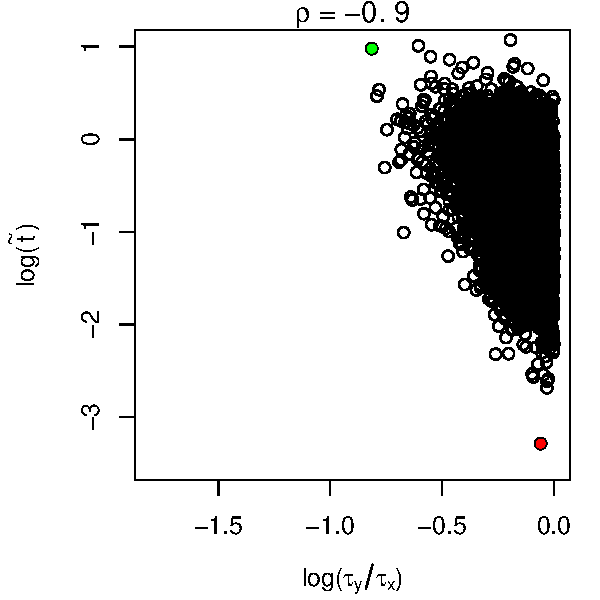
\includegraphics[width=1\linewidth]{small-sigma-t-scatterplot--09.pdf}
    \end{minipage}
    %% 
    & \begin{minipage}{0.3\textwidth}
      \centering
      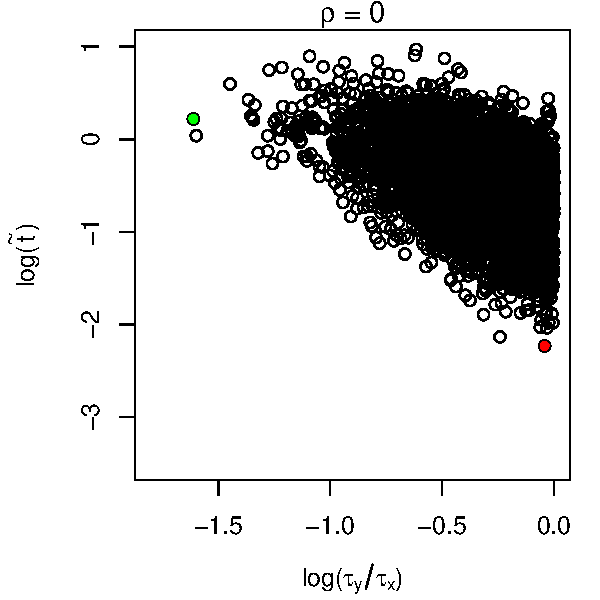
\includegraphics[width=1\linewidth]{small-sigma-t-scatterplot-0.pdf}
    \end{minipage}
    & \begin{minipage}{0.3\textwidth}
      \centering
      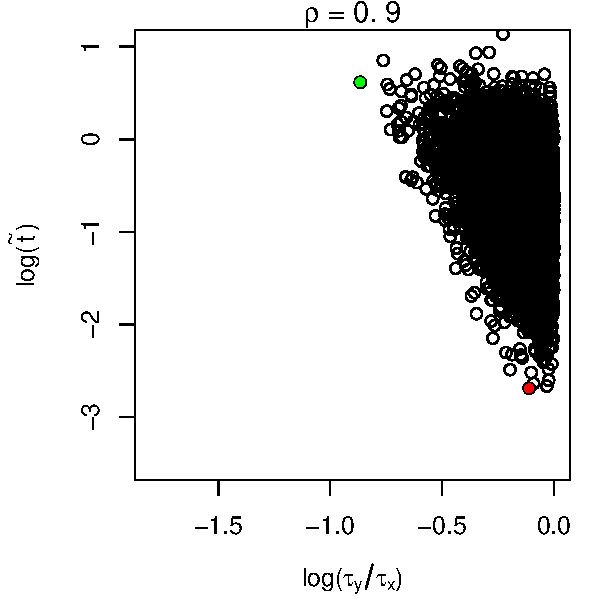
\includegraphics[width=1\linewidth]{small-sigma-t-scatterplot-09.pdf}
    \end{minipage}
  \end{tabular}
  \caption{Plots of normalized parameters $\log(\tilde{t})$
    vs. $\log(\tau_y/\tau_x)$ generated from processes with diffusion
    parameters sampled from
    $\log(\sigma_x) \overset{\mbox{\small i.i.d.}}{\sim} N(1,1)$ and
    $\log(\sigma_y) \overset{\mbox{\small i.i.d.}}{\sim} N(1,1)$ for
    three regimes of $\rho$. Combinations with smallest
    $\log(\tilde{t})$ (red) and $\log(\tau_y/\tau_x)$ (green). These
    points are candidates for having most problematic likleihood
    values.}
  \label{fig:small-sigma-y-t-samples}
\end{figure}
  We change the form of the basis functions in the Galerkin solution
  to account for different resolutions in the principal $x-$ and $y-$
  directions. The basis elements in (17) of Chapter 2 then become
  \begin{align}
    \psi_i(x,y) &= \frac{1}{2\pi \tilde{\sigma}_x \tilde{\sigma}_y \sqrt{1-\tilde{\rho}^2}}  \exp\left\{ -\frac{1}{2(1-\tilde{\rho}^2)} \left( \frac{(x - x_i)^2}{\tilde{\sigma}_x^2} - 2\tilde{\rho} \frac{(x-x_i)(y-y_i)}{\tilde{\sigma}_x\tilde{\sigma}_y} +  \frac{(y - y_i)^2}{\tilde{\sigma}_y^2}  \right)  \right\}
\end{align}
for some parameters
$(\tilde{\rho}, \tilde{\sigma}_x, \tilde{\sigma}_y)$ which together
control the resolution of the solution in the two principal
directions. The scheme used to set the node points over the
computational domain remains the same.

Any choice of basis-generating parameters
$(\tilde{\rho}, \tilde{\sigma}_x, \tilde{\sigma}_y)$ produces a finite
number of basis elements, meaning that there are lower bounds for
$\tau_y/\tau_x$ and $\tilde{t}$ which admit a valid solution. The new
normalized problem (\ref{eq:new-normalized}) conveniently provides a
computational tool for identifying how well the method can accommodate
difficult regions for likelihood computation, which are intuitively
associated with small $\tilde{t}$ and $\tau_y/\tau_x$. By generating
varying diffusion parameter combinations and observing the joint
distribution of the normalized parameters, we can identify extreme
combinations of $(\tilde{t}, \tau_y/\tau_x)$ parameter values. To do
so, we sample the original diffusion parameters $\sigma_x$ and
$\sigma_y$ independently from a heavy-tailed distribution in order to
capture cases where there is a several order magnitude difference
between $\sigma_x$ and $\sigma_y$. For our purposes, we sample
\begin{align}
  \log(\sigma_x) &\overset{\mbox{\small i.i.d.}}{\sim} N(1,1), &
  \log(\sigma_y) &\overset{\mbox{\small i.i.d.}}{\sim} N(1,1),
\end{align}
$5,000$ times then, for each pair of sampled values,
(\ref{eq:process-evolution}) is solved with a forward Euler
discretization (step $\Delta = 1\cdot 10^{-6}$); then the parameters
are normalized as in (\ref{eq:new-normalized}). The samples for
$\log(\tau_y/\tau_x)$ and $\log(\tilde{t})$ are shown in Figure
(\ref{fig:small-sigma-y-t-samples}). Across the three regimes of
$\rho$, extreme values for the normalized parameters are defined by
having either the smallest $\tau_y/\tau_x$ or $\tilde{t}$ in the
sample produced. These points are denoted by the the red and green
points in Figure (\ref{fig:small-sigma-y-t-samples}) and are
candidates for having a likelihood function which is smallest at those
extreme values and may be most problematic to resolve with respect to
our Galerkin solution. An intersting observation is that there is a
tradeoff between the size of $\tau_y/\tau_x$ and $\tilde{t}$. In other
words, it is very unlikely to encounter data points generated by a
diffusion equation having $(\tau_y/\tau_x, \tilde{t})$ in the
lower-left corner of the parameter space.

\begin{figure}
  \centering
  \begin{tabular}{ccc}
    \begin{minipage}{0.33\textwidth}
      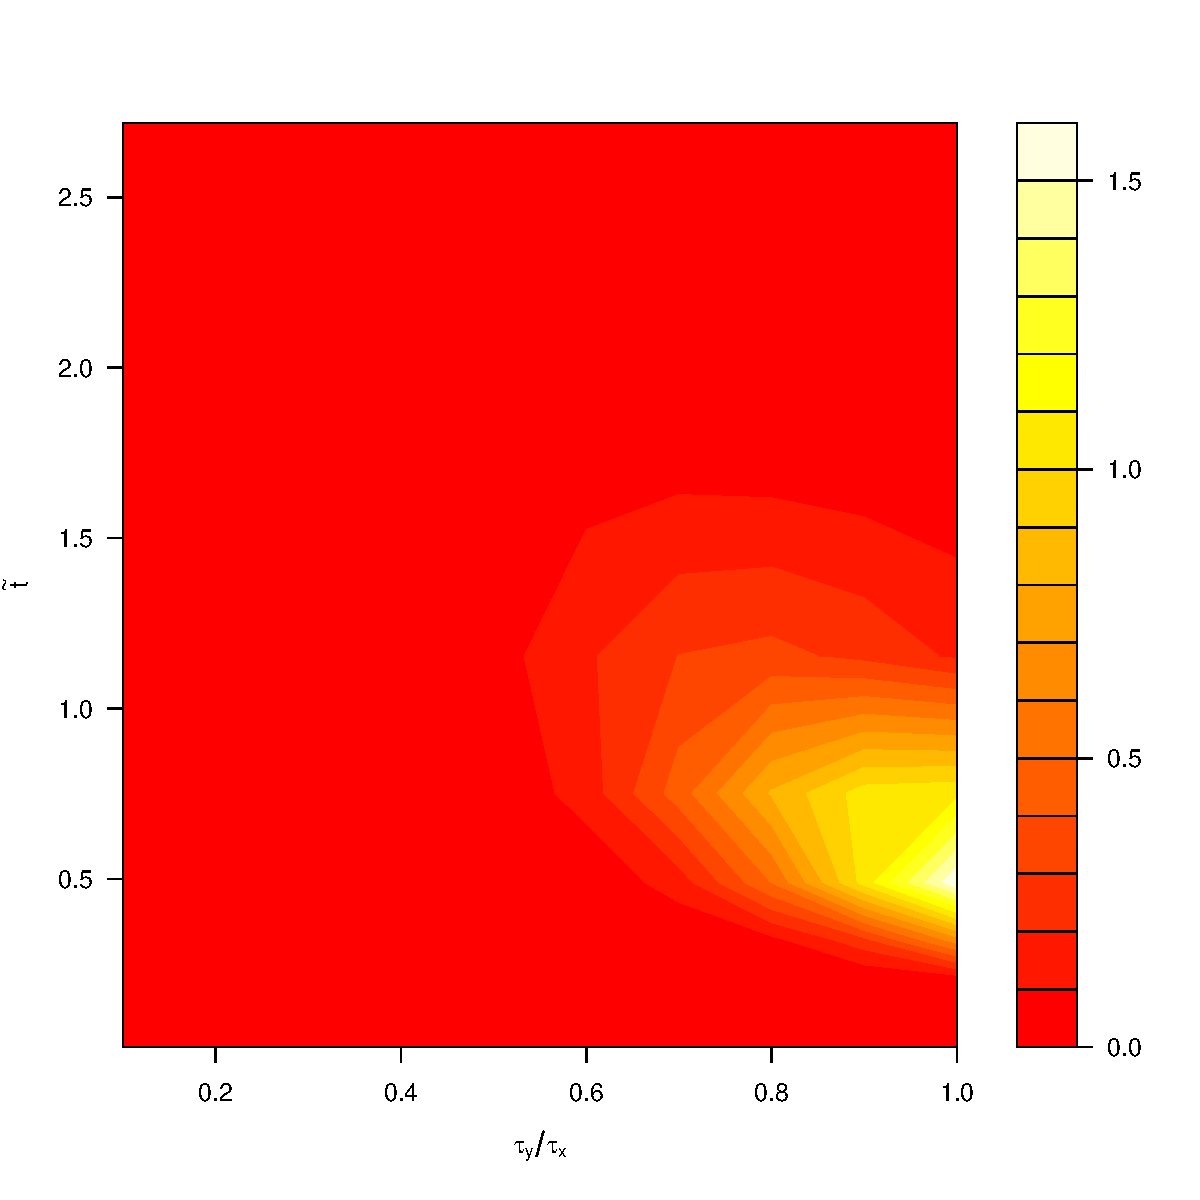
\includegraphics[width=1\linewidth]{small-sigma-analytic.pdf}
    \end{minipage}
    &
      \begin{minipage}{0.33\textwidth}
      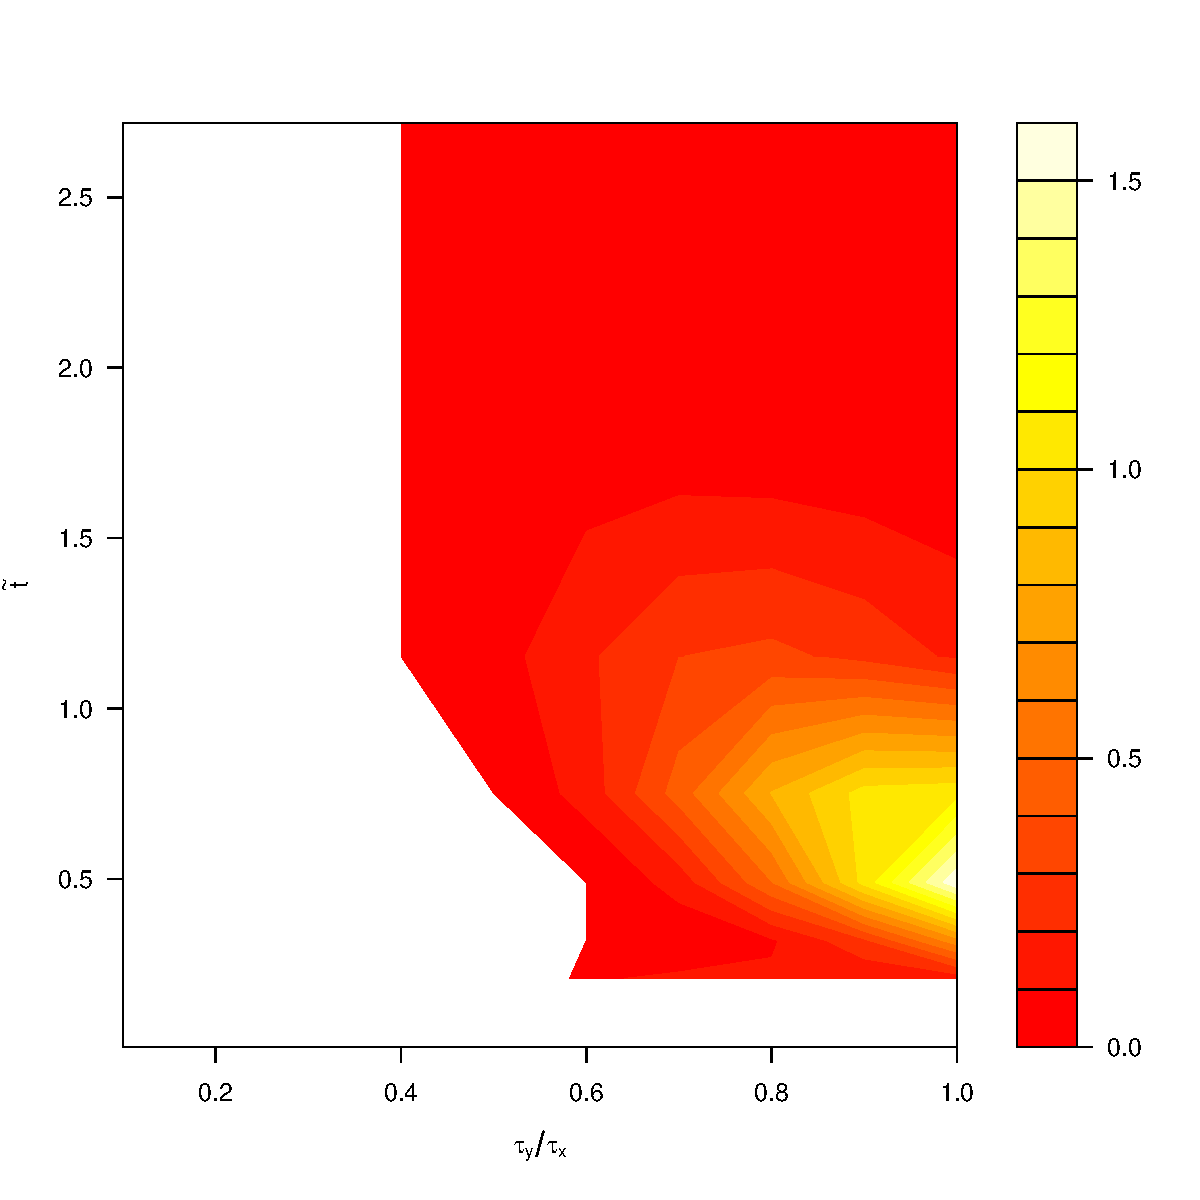
\includegraphics[width=1\linewidth]{small-sigma-Galerkin-no-filter.pdf}
    \end{minipage}
      & \begin{minipage}{0.33\textwidth}
      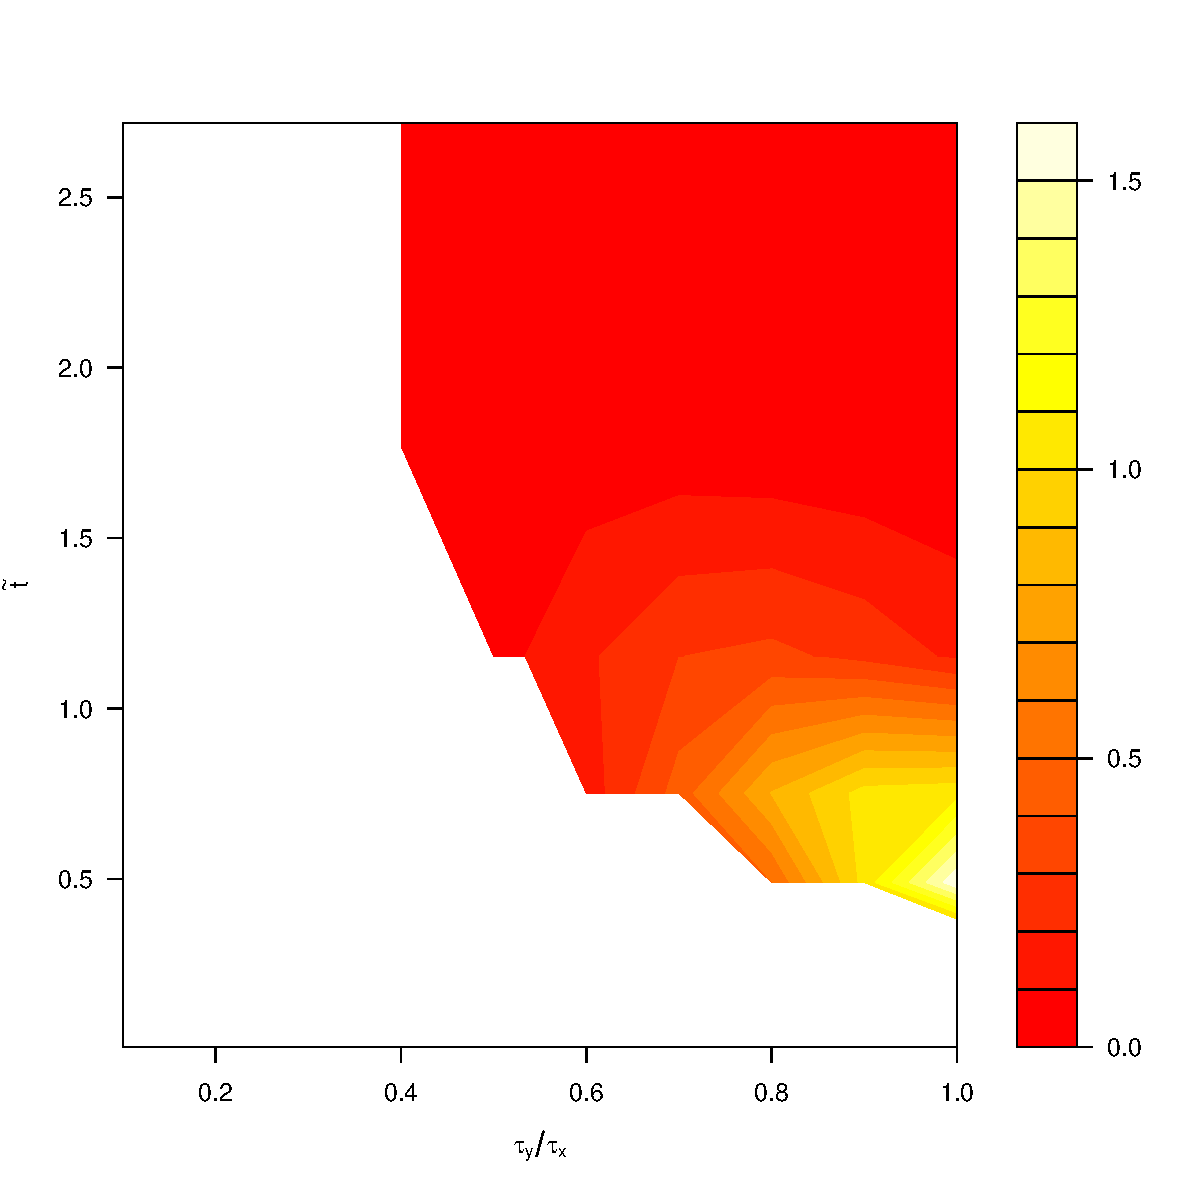
\includegraphics[width=1\linewidth]{small-sigma-Galerkin.pdf}
    \end{minipage}
  \end{tabular}
  \caption{Likelihood surfaces for small-$\tau_y/\tau_x$ (green) point
    from the $\rho = 0$ regime. Left panel shows the analytic solution
    for the likelihood. The middle panel includes the Galerkin
    solution where lack of color denotes parameter combinations which
    yield a negative (inadmissible) solution. The right panel shows
    the Galerkin solution where blank points denote instances where
    the Galerkin solution differs from the analytic solution by more
    than 5\%. The basis parameters used are $\tilde{\sigma}_x = 0.3$,
    $\tilde{\sigma}_y = 0.1$ and $\tilde{\rho} = 0$.}
  \label{fig:small-sigma-sol}
\end{figure}
The quality of the Galerkin solution in the $\rho \neq 0$ cases cannot
be directly assessed because of a lack of a closed-form analytic
solution. However, this is not the case for $\rho=0$. Figure
(\ref{fig:small-sigma-sol}) features both the analytic and Galerkin
likelihood surfaces for the small $\tau_y/\tau_x$ (green) point in
Figure (\ref{fig:small-sigma-y-t-samples}). The basis parameters used
to generate the Galerkin solution in this case are
$\tilde{\sigma}_x = 0.3, \tilde{\sigma}_y = 0.1, \tilde{\rho} =
0$. The left panel shows the true analytic solution; the middle panel
shows the Galerkin solution, where lack of color signifies a negative
value produces for the likelihood. This is automatically an
inadmissible solution. Finally, the right panel shows the Galerkin
solution where likelihood values differing from the true solution by
more than 5\% have been discarded. We see that the Galerking solution
fails in cases where $\tilde{t}$ or $\tau_y/\tau_x$ approach small
values relative to the values of the likelihood function. Figure
(\ref{fig:small-t-sol}) similarly shows the likelihood surface for the
small $\tilde{t}$ (red) point in Figure
(\ref{fig:small-sigma-y-t-samples}). We see that the choice of basis
parameters for the $\rho = 0$ case is capable of resolving the main
probability mass in the likelihood function for both extreme cases
considered.
\begin{figure}
  \centering
  \begin{tabular}{ccc}
    \begin{minipage}{0.33\textwidth}
      \centering
      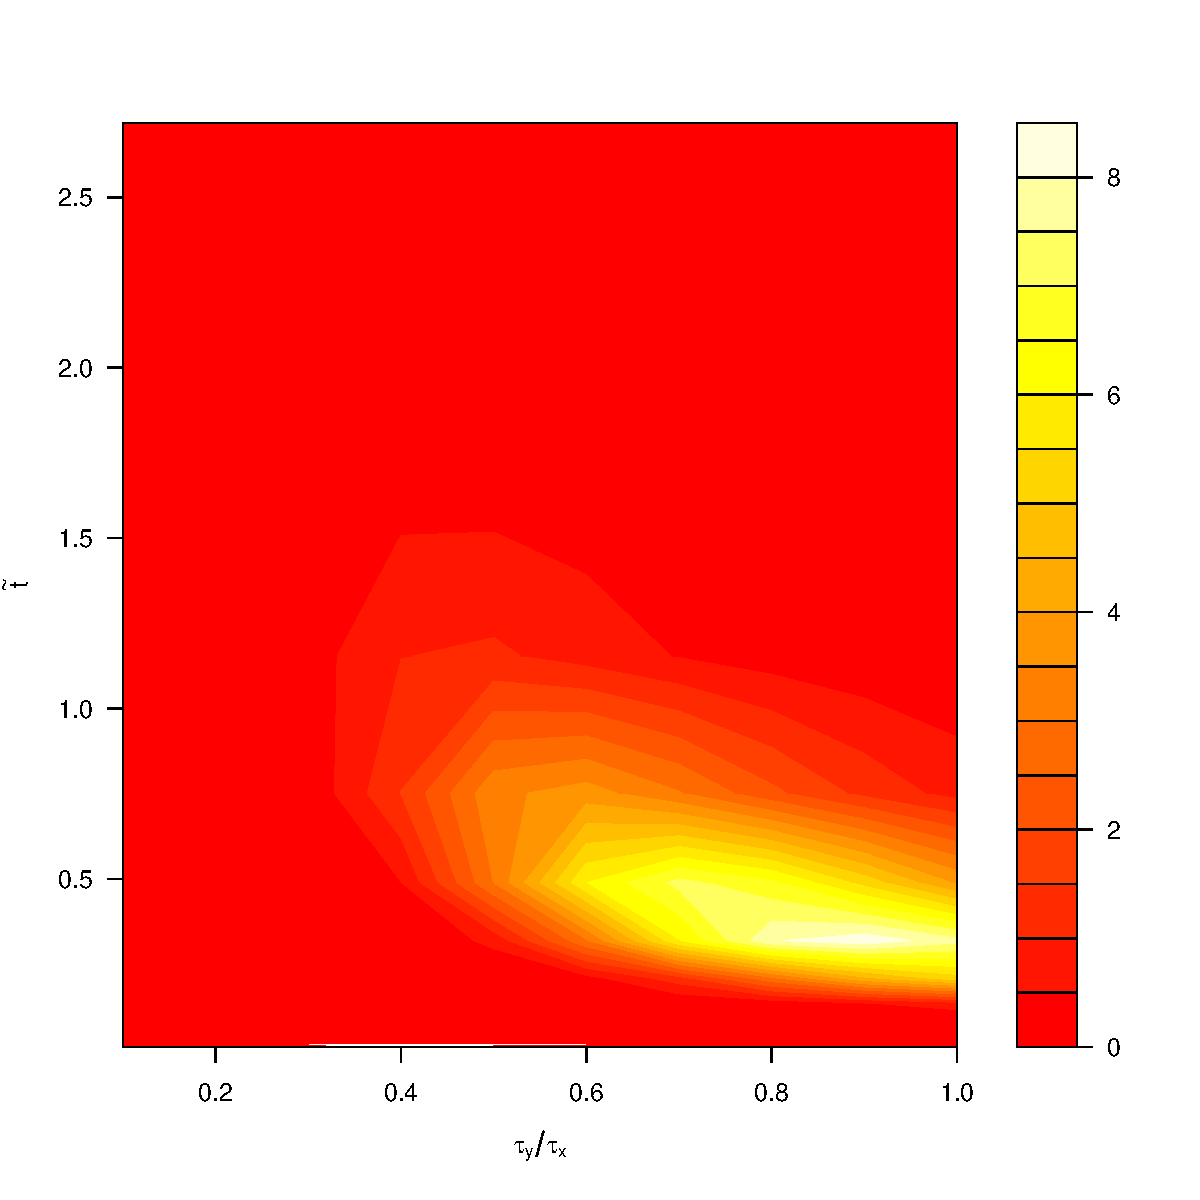
\includegraphics[width=1\linewidth]{small-t-analytic.pdf}
    \end{minipage}
    %% 
    & \begin{minipage}{0.33\textwidth}
      \centering
      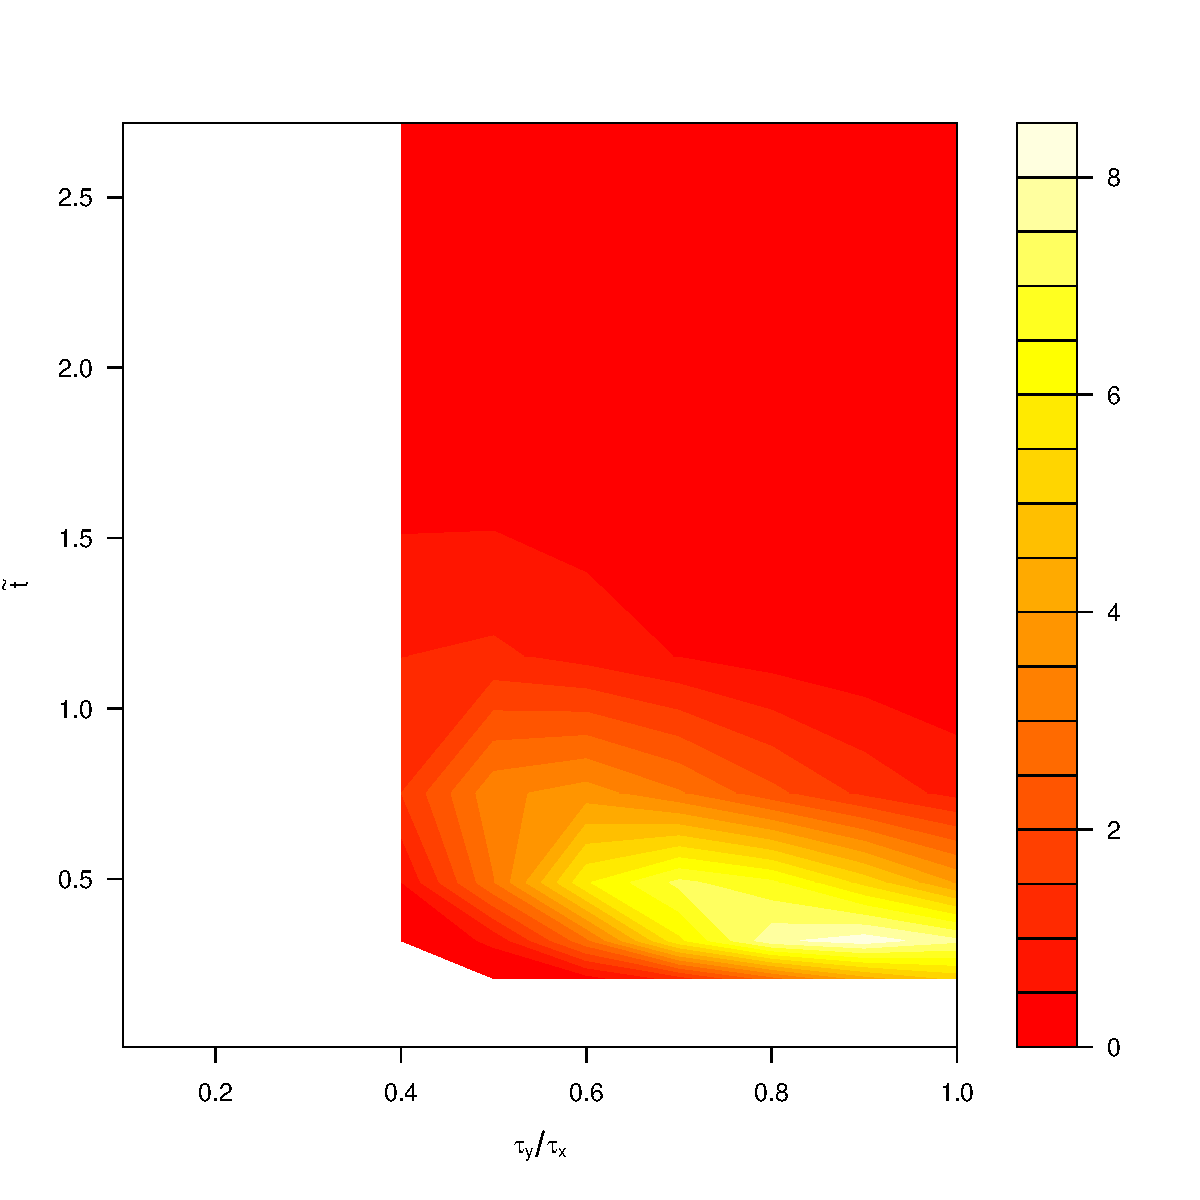
\includegraphics[width=1\linewidth]{small-t-Galerkin-no-filter.pdf}
    \end{minipage}
    & \begin{minipage}{0.33\textwidth}
      \centering
      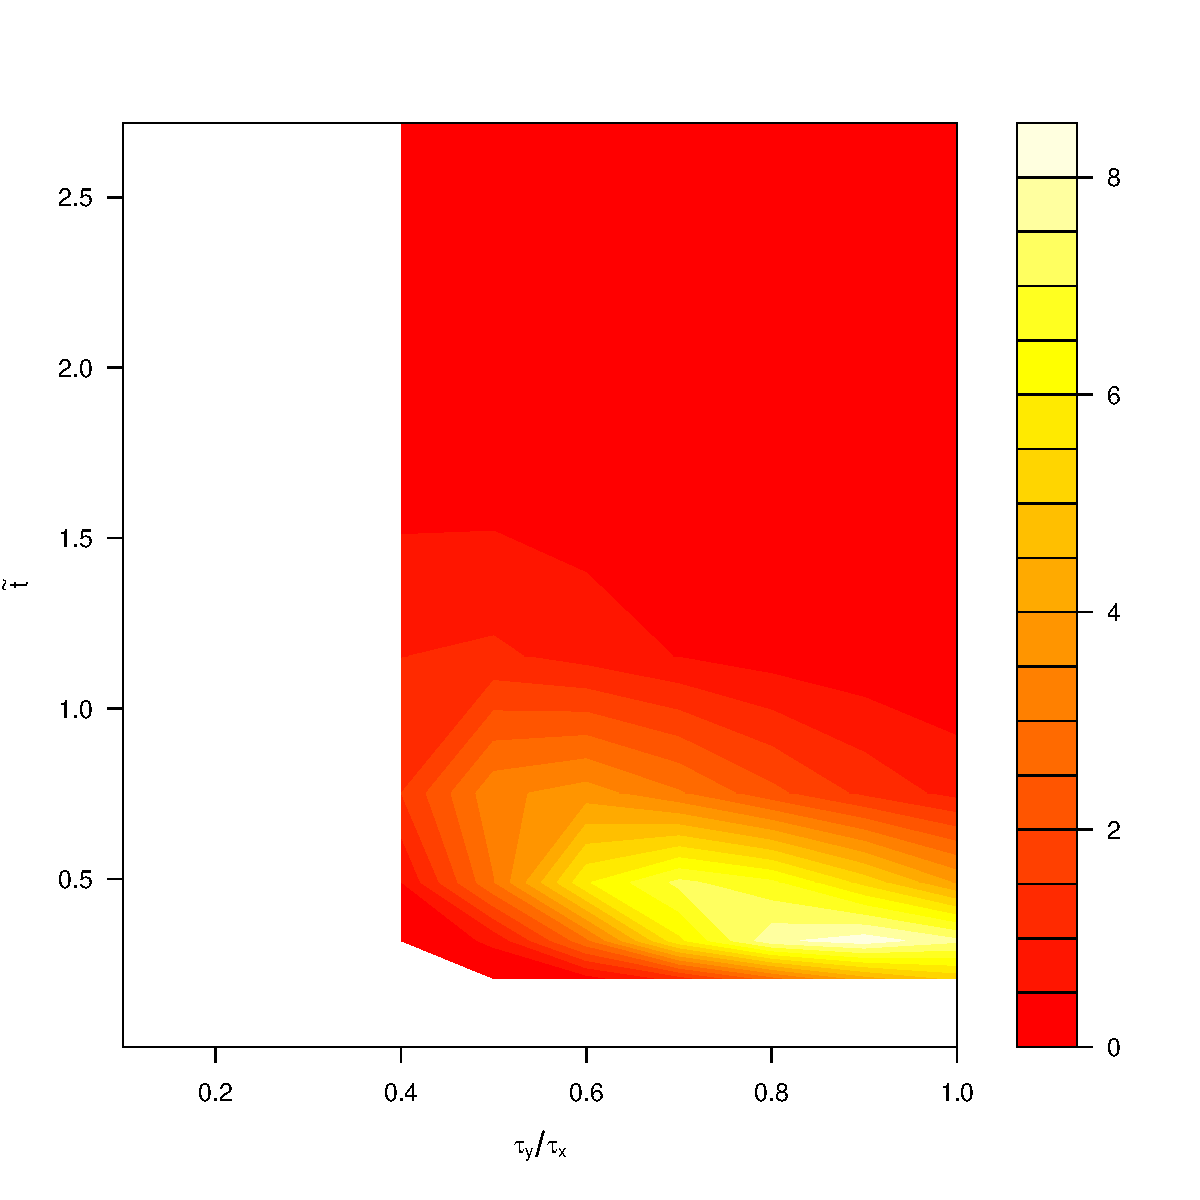
\includegraphics[width=1\linewidth]{small-t-Galerkin-no-filter.pdf}
    \end{minipage}
  \end{tabular}
  \caption{Likelihood surfaces for small-$\tilde{t}$ (red) point
    from the $\rho = 0$ regime. Left panel shows the analytic solution
    for the likelihood. The middle panel includes the Galerkin
    solution where lack of color denotes parameter combinations which
    yield a negative (inadmissible) solution. The right panel shows
    the Galerkin solution where blank points denote instances where
    the Galerkin solution differs from the analytic solution by more
    than 5\%. The basis parameters used are $\tilde{\sigma}_x = 0.3$,
    $\tilde{\sigma}_y = 0.1$ and $\tilde{\rho} = 0$.}
  \label{fig:small-t-sol}
\end{figure}


A hard cutoff for the Galerkin solution for $\tilde{t} \geq 0.25$ and
$\tau_y/\tau_x \geq 0.4$ is sufficient to capture the main probability
mass of the likelihood surface. This was confirmed by computing the
surface for all other samples in the middle panel of Figure
(\ref{fig:small-sigma-y-t-samples}). From an empirical standpoint this
is also the case when $\rho \neq 0$. Figure (\ref{fig:rho-09}) shows
the likelihood surfaces for the extreme parameter combinations where
$\rho = 0.9$, with parameters used for the basis generation being
$\tilde{\sigma}_x = 0.3$, $\tilde{\sigma}_y = 0.1$ and
$\tilde{\rho} = 0.7,$ for the small $\tilde{t}$ (green) and
small-$\tau_y/\tau_x$ (red) points of the right panel in Figure
(\ref{fig:small-sigma-y-t-samples}). The solution generated has
properties consisent with those of the analytic $\rho=0$ solution:
conditional on either $\tau_y/\tau_x$ or $\tilde{t}$, the solution
formed, when valid, exhibits unimodality, and the main probability
mass of the likelihood is bounded by $\tilde{t} \geq 0.25$ and
$\tau_y/\tau_x \geq 0.4$.

\begin{figure}
  \centering
  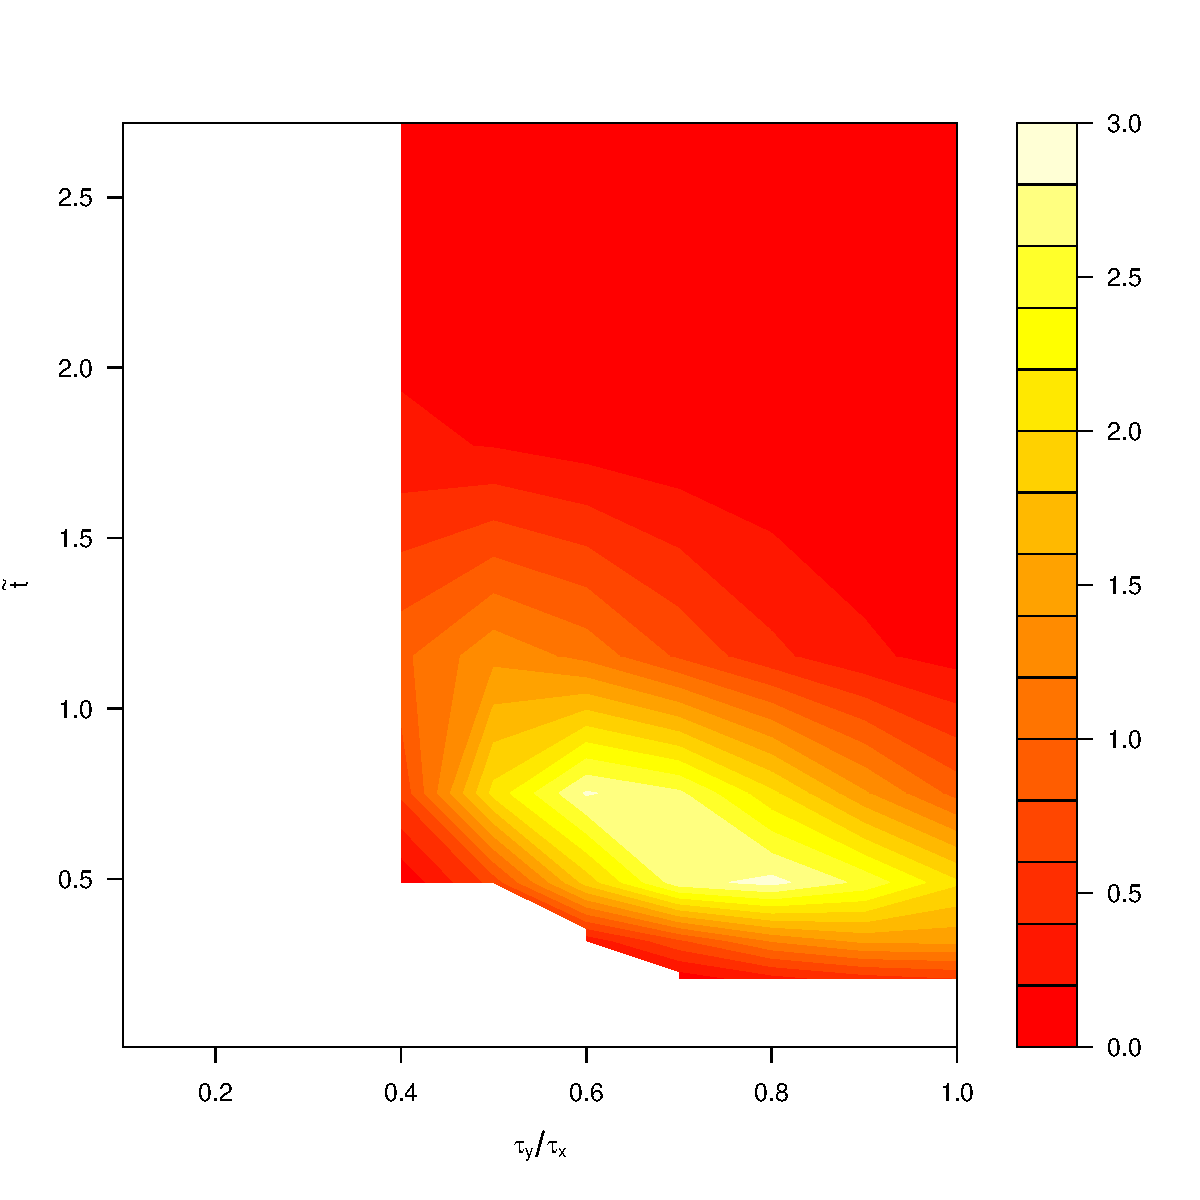
\includegraphics[scale=0.3]{small-sigma-Galerkin-no-filter-rho-09.pdf}
  \caption{.}
  \label{fig:rho-09}
\end{figure}
To further corroborate our empirical findings with respect to the
bounds on the probability mass of the likelihood, we consider the
analytic solution for the problem when $\tilde{t} << 1$. We have
already introduced such a small-time solution in Chapter 2
and only modify it by considering a system of images defined not by a
single reflection, but by a reflection about each of the four
boundaries. This produces a system of 16 images of the fundamental
solution to the heat equation in (\ref{eq:new-normalized}), which is a
bivariate Gaussian with the given diffusion parameters.  We assume
that the small-time $\tilde{t}_{\varepsilon}$ is small enough such
that the boundary conditions are enforced numerically, which is the
case for the previously defined $\tilde{t}_\varepsilon$. This produces
a solution to the governing equation explicitly differentiable with
respect to the boundaries and having the form
  \begin{align}
    p(x,y,\tilde{t}_\varepsilon) &= \phi(x,y | x_0, y_0, 1, \tau_y/\tau_x, \rho) + \sum_{k' =1}^K
                                   w_{k'} \phi(x,y | x_{k'}, y_{k'}, 1, \tau_y/\tau_x, \rho),
  \end{align}
  where $\phi(x,y | x_k, y_k, 1, \tau_y/\tau_x, \rho)$ is the
  bivariate Gaussian
  \begin{align}
    \phi(x,y | x_k, y_k, 1, \tau_y/\tau_x, \rho) &= \frac{1}{2\pi \tilde{t}_\varepsilon \tau_y/\tau_x \sqrt{1-\rho^2}}  \exp\left\{ -\frac{1}{2(1-\rho^2)\tilde{t}_\varepsilon} \left( \frac{(x - x_k)^2}{1} - 2\rho \frac{(x-x_k)(y-y_k)}{\tau_y/\tau_x} +  \frac{(y - y_k)^2}{\tau_y^2/\tau_x^2}  \right)  \right\},
  \end{align}
  $K=15$, $(x_0, y_0)$ is the initial condition for the problem, and
  $w_k$ is either $1$ or $-1$. In the images solution, only the
  location parameters for $\phi$ are functions of the boundaries, and
  only one of the images has location parameters $(x_k, y_k)$ as functions of all four
  boundaries. Thus, upon differentiation, the small-time likelihood
  becomes
    \begin{align}
      &\frac{\partial^4}{\partial a_x \partial b_x \partial a_y \partial b_y}p(x,y,\tilde{t}_\varepsilon) = \nonumber \\
      &\frac{\partial^4}{\partial a_x \partial b_x \partial a_y \partial b_y} \left( \frac{1}{2\pi \tilde{t}_\varepsilon \tau_y/\tau_x \sqrt{1-\rho^2}}  \exp\left\{ -\frac{1}{2(1-\rho^2)\tilde{t}_\varepsilon} \left( \frac{(x - x_k)^2}{1} - 2\rho \frac{(x-x_k)(y-y_k)}{\tau_y/\tau_x} +  \frac{(y - y_k)^2}{\tau_y^2/\tau_x^2}  \right)  \right\} \right).
    \end{align}
    Viewing the likelihood as a function of $\tilde{t}_\varepsilon$
    and $\tau_y^2/\tau_x^2$ and carrying out the differentiation
    yields a likelihood proportional to an inverse Gamma-like
    probability distribution
    \begin{align}
      &L(\tilde{t}_\varepsilon, \tau_y^2/\tau_x^2 | \rho) \nonumber \\
      &\propto \frac{1}{\tilde{t}_\varepsilon^5}\left(\frac{1}{(\tau_y^2/\tau_x^2)^{9/2}} + C_1 \frac{1}{(\tau_y^2/\tau_x^2)^{8/2}} + \cdots + C_8 \frac{1}{(\tau_y^2/\tau_x^2)^{1/2}} \right) \exp\left\{ -\frac{1}{2(1-\rho^2)\tilde{t}_\varepsilon} \left( \frac{(x - x_k)^2}{1} - 2\rho \frac{(x-x_k)(y-y_k)}{\tau_y/\tau_x} +  \frac{(y - y_k)^2}{\tau_y^2/\tau_x^2}  \right)  \right\} . \label{eq:inv-Gam-likelihood}
    \end{align}
    % This further reduces in the $\rho = 0$ case, where
    %     \begin{align}
    %   L(\tilde{t}_\varepsilon, \tau_y^2/\tau_x^2 | \rho = 0) &\propto \frac{1}{\tilde{t}_\varepsilon^5}\left(\frac{1}{(\tau_y^2/\tau_x^2)^{9/2}}\right) \exp\left\{ -\frac{1}{2\tilde{t}_\varepsilon} \left( \frac{(x - x_k)^2}{1} +  \frac{(y - y_k)^2}{\tau_y^2/\tau_x^2}  \right)  \right\}. \label{eq:inv-Gam-likelihood-no-rho}
    % \end{align}
    % Since the method of images is valid for $\rho=0$, the likelihood
    % is proportional to a linear combination of inverse Gamma
    % distributions when considering a general $\tilde{t}$.

    Viewing (\ref{eq:inv-Gam-likelihood}) as a function of
    $\tilde{t}_\varepsilon$ alone, we have
    \begin{align*}
      L(\tilde{t}_\varepsilon | \tau_y^2/\tau_x^2, \rho) &\propto
                                                           \frac{1}{\tilde{t}_\varepsilon^5} \exp\left\{
                                                           -\frac{1}{2(1-\rho^2)\tilde{t}_\varepsilon} \left( \frac{(x -
                                                           x_k)^2}{1} - 2\rho \frac{(x-x_k)(y-y_k)}{\tau_y/\tau_x} +
                                                           \frac{(y - y_k)^2}{\tau_y^2/\tau_x^2} \right) \right\} \\
                                                         &\propto IG\left( \tilde{t}_\varepsilon | \alpha = 4, \beta = \frac{1}{2(1-\rho^2)} \left( \frac{(x -
                                                           x_k)^2}{1} - 2\rho \frac{(x-x_k)(y-y_k)}{\tau_y/\tau_x} +
                                                           \frac{(y - y_k)^2}{\tau_y^2/\tau_x^2} \right)\right)
      \end{align*}
      Since the image $k$ is reflected once about each boundary, both
      $(x-x_k), (y-y_k) \geq 1$ and combining with the bound $\tau_y/\tau_x \leq 1$,
      \[
        \beta \geq \frac{1}{2(1-\rho^2)} \left( 1 - 2\rho
          \frac{1}{\tau_y/\tau_x} + \frac{1}{\tau_y^2/\tau_x^2}
        \right) \geq \frac{3}{2}.
      \]
      Then the mode for the inverse Gamma-like likelihood, conditional on
      $\tau_y/\tau_x$ and $\rho$, is bounded below by
      \[
        \frac{\beta}{\alpha+1} \geq 0.3.
      \]
      The $\tilde{t}$ likelihood approximately follows an inverse
      Gamma distribution with mode greater than or equal to about
      $1/3$ within the small-time regions of the parameter space. This
      functional relationship changes outside the small-time region,
      but it still dominates the likelihood. Although not true in
      general, increasing $\tilde{t}$ away from the small-time region
      can be accomodated with additional reflections of the system of
      images about the boundaries. The new images add to the
      likelihood for $\tilde{t}$, but their contribution decays
      exponentially compared the nearest term to the computational
      domain (which is image $k$ in (\ref{eq:inv-Gam-likelihood})) since they
      scale away linearly as a function of the number of reflections.

      A similar analysis can be performed for $(\tau_x/\tau_y)^2$, where $\alpha \leq 7/2$ and 
      \[
        \beta \geq \frac{(y-y_k)}{2(1-\rho^2)\tilde{t}_\varepsilon} \geq \frac{1}{2\tilde{t}_\varepsilon}.
      \]
      Hence, the mode for the likelihood as a function of
      $\tau_y/\tau_x$ conditional on $\rho$ is bounded by
      \[
        \sqrt{\frac{\beta}{\alpha+1}} \geq \sqrt{\frac{1}{7\tilde{t}_\varepsilon}} \geq 0.33.
      \]

      The above derived bounds for where the main probability mass of
      the likelihood abides within the parameter space corroborates
      our empirical observations, and they also further support our
      choice for basis parameters and their capability of resolving
      the main parts of the likelihood surface.

      So far we have demonstrated that a choice of basis function
      parameters can reasonably resolve the main probability mass in
      the likelihood function over the parameter space of the
      normalized problem. However, the solution does explicitly fail
      away from the main probability mass of the likelihood. To
      evaluate the likelihood in such conditions, we introduce an
      analytic extension of our numerical solution.

    \item The analytic extension to our numerical method is motivated
      by (\ref{eq:inv-Gam-likelihood}). We use an inverse Gamma
      approximation to the likelihood in inadmissible regions of the
      parameter space. We extend into either the small $\tilde{t} < 0.25$ or
      small $\tau_y/\tau_x < 0.40$ regions by fitting the function
      \[
        f(x) = C\, x^{-\alpha-1} \exp\left( -\frac{\beta}{x} \right)
      \]
      using three valid likelihood points with bigger $\tilde{t}$ or
      $\tau_y/\tau_x$ values. For points falling in the small
      parameter region for both $\tilde{t}$ and $\tau_y/\tau_x$, we
      first approximate likelihood values into one then the other
      regions. Although more computationally intensive, this
      correction allows us to validly approximate likelihoods in the
      parameter space for the normalized problem that cannot be
      resolved by our Galerkin solution.

      Our method is illustrated in Figure (\ref{eq:extrapolating})
      below. The left panel shows the analytic and extended Galerkin
      likleihoods over the range for $\tilde{t}$

      \begin{figure}
        \centering
        \includegraphics[scale=0.5]{small-sigma-extrapolation-rho-0.pdf}
        \caption{.}
        \label{fig:extrapolation}
      \end{figure}
      
    \end{enumerate}


\section{Particle Filtering}
Bayesian approaches for estimating complex hierarchical models like
those in (\ref{eq:process-evolution}) -
(\ref{eq:correlation-evolution}) are common. The primary focus of such
inferential algorithms is the generation of dependent samples from the
posterior distributions of model parameters and unobservable latent
trajectories via Markov Chain Monte Carlo (MCMC). However, the highly
non-linear nature of the state-space model considered here prohibits
conditional Gaussian representations and thereby limits the
application of MCMC methods. Instead, we use a particle filtering
approach, which is a particular version of a sequential Monte Carlo
algorithm (see \cite{doucet2001sequential} for an overview), to
generate samples from the posterior distribution of the collection of
time-dependent parameters, which we abbreviate to
\[
  \sigma_t := (\sigma_{x,t}, \sigma_{y,t}, \rho_t),
\]
as well as all of the time-constant parameters governing the evolution
of the process, which we transform to be on the $(-\infty, \infty)$
scale and denote
\[
  \phi := (\alpha_x, \alpha_y, \alpha_\rho, \theta_x, \theta_y,
  \theta_\rho, \log(\tau_x), \log(\tau_y), \log(\tau_\rho),
  \mbox{logit}(\rho_x), \mbox{logit}(\rho_y)).
\]
Most sequential Monte Carlo algorithms assume the structural
parameters $\phi$ to be known and fixed, which is not the case for the
considered problem. We therefore follow \cite{rodriguez2012} and use a
version of the augmented particle filter of \cite{pitt1999filtering}
developed by \cite{liu2001combined} to sample from the full
posterior.

Particle filters use a discrete mixture to represent the posterior
distribution $p(\sigma_t, \phi | \mathcal{D}_t)$, where
$\mathcal{D}_t$ represents all of the observable information up to
time $t$:
\[
  \mathcal{D}_t = (x_0, y_0, a_{x,\Delta}, b_{x,\Delta}, a_{y,\Delta},
  b_{y,\Delta}, x_\Delta, y_\Delta, \ldots, x_{t-\Delta},
  y_{t-\Delta}, a_{x,t}, b_{x,t}, a_{y,t}, b_{y,t}, x_t, y_t).
\]
In this mixture approximation, the information about the parameters
given the current data is captured in the parameter values and weights
associated with each particle:
\[
  p(\sigma_t, \phi | \mathcal{D}_t) \approx \sum_{k=1}^K \delta(\sigma_t^{(k)} - \sigma_t) \delta(\phi^{(k)} - \phi) w_t^{(k)}
\]
Given this approximation of $p(\sigma_t, \phi | \mathcal{D}_t)$,
additional information at time $t+\Delta$ is incorporated by updating
each particle weight and parameter values via an appropriately chosen
importance sampling distribution and Bayes' Theorem. In the case of
the augmented particle filter of \cite{pitt1999filtering}, which
treats the structural parameters $\phi$ are known and fixed, the
approximate distribution of the state of the system at time $t$ is
\[
  p(\sigma_t | \phi, \mathcal{D}_t) \approx \sum_{k=1}^K
  \delta(\sigma_t^{(k)} - \sigma_t) w_t^{(k)};
\]
the posterior $p(\sigma_{t+\Delta} | \phi, \mathcal{D}_{t+\Delta})$ is
\textit{augmented} with the particle index $k$ and sampled with Bayes' Theorem:
\begin{align}
  p(\sigma_{t+\Delta}, k | \phi, \mathcal{D}_{t+\Delta}) &\propto
                                                           p(x_{t+\Delta}, y_{t+\Delta}, a_{x,t+\Delta}, b_{x, t+\Delta},
                                                           a_{y,t+\Delta}, b_{y, t+\Delta} | \sigma_{t+\Delta}, k, \phi,
                                                           \mathcal{D}_t)p(\sigma_{t+\Delta},k | \phi, \mathcal{D}_t), \\
                                                         &= p(\mathbf{y}_{t+\Delta} | \sigma_{t+\Delta}, \phi, \mathcal{D}_t) p(\sigma_{t+\Delta} | \sigma_{t}^{(k)}, \phi) w^{(k)}_t. \label{eq:augmented-posterior}
\end{align}
\cite{pitt1999filtering} sample the joint posterior with a proposal
distribution which replaces $\sigma_{t+\Delta}$ with a representative
value in the one-step predictive distribution
$p(\sigma_{t+\Delta} | \sigma_t^{(k)}, \phi)$, such as the predictive
mean. In this way $k$ is sampled then $\sigma_{t+\Delta}$ from the
predictive distribution conditional on $k$. The new weight
$w_{t+\Delta}^{(k)}$ is proportional to the ratio of the sampled
$\sigma_{t+\Delta}$ and representative value in the likelihood for the
data.


\cite{liu2001combined} extend the augemented particle filter of
\cite{pitt1999filtering} to allow for the estimation of the constant
structural parameter $\phi$. This is done by introducing an artificial
evolution for the fixed parameter, which is now indexed by $t$, and
defining the transition density
\[
  p(\phi_{t+\Delta} | \mathcal{D}_t) \approx \sum_{k=1}^K
  N(\phi_{t+\Delta} | a\phi_t^{(k)} + (1-a)\bar{\phi}_t, (1-a^2)^2 V_t),
\]
where $a$ is a discount factor between 0 and 1, $\bar{\phi}_t$ is the
average of samples for $\phi$ at $t$ and $V_t$ is the respective
sample covariance at time $t$. The Gaussian perturbation of $\phi_t$
is appropriate, as we have transformed each of the structural
parameters to $\mathbb{R}$, while the shrinkage kernel approximation
preserves the mean and covariance structure of the posterior
distribution from $t$ to $t+\Delta$. This limits the injection of
entropy into the system that would otherwise occur with simpler,
conditionally independent Gaussian perturbations.

The augmented posterior then becomes
\begin{align}
  p(\sigma_{t+\Delta}, \phi_{t+\Delta}, k | \mathcal{D}_{t+\Delta}) \propto p(\mathbf{y}_{t+\Delta} | \sigma_{t+\Delta}, \phi_{t+\Delta}, \mathcal{D}_t) p(\sigma_{t+\Delta} | \phi_{t+\Delta}, \sigma_{t}^{(k)}, \mathcal{D}_t)N(\phi_{t+\Delta} | a\phi_t^{(k)} + (1-a)\bar{\phi}_t, (1-a^2)^2 V_t) w^{(k)}_t. \label{eq:augmented-posterior-liu}
\end{align}
Sampling from the posterior (\ref{eq:augmented-posterior-liu}) is also
done with via a proposal where $(\sigma_{t+\Delta}, \phi_{t+\Delta})$
are replaced with predictive means conditional on $k$ in the
likelihood:
\begin{align}
  p(\sigma_{t+\Delta}, \phi_{t+\Delta}, k | \mathcal{D}_{t+\Delta}) &= p(\mathbf{y}_{t+\Delta} | E[\sigma_{t+\Delta} | \sigma_{t}^{(k)}, \phi_t^{(k)}], a\phi_t^{(k)} + (1-a)\bar{\phi}_t) \nonumber \\
  & \times p(\sigma_{t+\Delta} | \phi_{t+\Delta}^{(k)}, \sigma_{t}^{(k)}) N(\phi_{t+\Delta} | a\phi_t^{(k)} + (1-a)\bar{\phi}_t, (1-a^2)^2 V_t) w^{(k)}_t. \label{eq:proposal-liu}
\end{align}
With (\ref{eq:proposal-liu}), we can integrate out
$(\sigma_{t+\Delta}, \phi_{t+\Delta})$ to propose $k$, then sample the
two remaining parameters respectively. The new weights are computed as
the likelihood ratio of the likelihood function. If we denote the
predictive means to be
\begin{align}
  m^{(k)}_{t+\Delta} &:= E[\sigma_{t+\Delta} | \sigma_{t}^{(k)}, \phi_t^{(k)}], \\
  \mu^{(k)}_{t+\Delta} &:= E[\phi_{t+\Delta} | k, \mathcal{D}_t] = a\phi_t^{(k)} + (1-a)\bar{\phi}_t,
\end{align}
our proposal distribution can be written as
\begin{align}
  p(\sigma_{t+\Delta}, \phi_{t+\Delta}, k | \mathcal{D}_{t+\Delta}) &= p(\mathbf{y}_{t+\Delta} | m^{(k)}_{t+\Delta}, \mu^{(k)}_{t+\Delta}) \nonumber \\
  & \times p(\sigma_{t+\Delta} | \phi_{t+\Delta}^{(k)}, \sigma_{t}^{(k)}) N(\phi_{t+\Delta} | \mu_{t+\Delta}^{(k)}, (1-a^2)^2 V_t) w^{(k)}_t. \label{eq:proposal-liu-2}
\end{align}
The steps in the particle filtering scheme are explicitly
\begin{enumerate}[1)]
\item Sample the particle indicator $k$ from the marginal proposal
  \[
    p(k| \mathcal{D}_{t+\Delta})= \displaystyle
    \int_{\sigma_{t+\Delta}} \displaystyle \int_{\phi_{t+\Delta}}
    p(\sigma_{t+\Delta}, \phi_{t+\Delta}, k | \mathcal{D}_{t+\Delta})
    d\sigma_{t+\Delta} \,d\phi_{t+\Delta} \propto p(\mathbf{y}_{t+\Delta} | m^{(k)}_{t+\Delta}, \mu^{(k)}_{t+\Delta}) w^{(k)}_t.
  \]
\item Conditional on $k$, sample $(\sigma_{t+\Delta}, \phi_{t+\Delta})$ from
  \begin{align*}
    \phi_{t+\Delta}^{(k)} &\sim N(\phi_{t+\Delta} | \mu_{t+\Delta}^{(k)}, (1-a^2)^2 V_t), \\
    \sigma_{t+\Delta}^{(k)} &\sim p(\sigma_{t+\Delta} | \phi_{t+\Delta}^{(k)}, \sigma_{t}^{(k)}).
  \end{align*}
\item Compute the new weight as the ratio of likelihoods:
  \begin{align*}
    w_{t+\Delta}^{(k)} \propto \frac{p(\mathbf{y}_{t+\Delta} | \sigma^{(k)}_{t+\Delta}, \phi^{(k)}_{t+\Delta})}{p(\mathbf{y}_{t+\Delta} | m^{(k)}_{t+\Delta}, \mu^{(k)}_{t+\Delta})}
  \end{align*}
\end{enumerate}
Steps 1) and 3) require a reliable way to compute the likelihood for
the observed process. This is particularly true in instances where
proposed and predictive values for the parameters are very unlikely
given the observation $\mathbf{y}_{t+\Delta}$. The finite precision of
the method we developed to compute the likelihood, mainly arising from
the truncation of the basis expansion of the solution, may yield
negative values for the likelihood. The ad-hoc correction of replacing
such values with numerically zero but positive values can yield
deleterious results, as what would otherwise be a small value for
$w_{t+\Delta}^{(k)}$ may be replaced with unity in the case where the
likelihood computation fails when evaluating both
$p(\mathbf{y}_{t+\Delta} | \sigma^{(k)}_{t+\Delta},
\phi^{(k)}_{t+\Delta})$ and
$p(\mathbf{y}_{t+\Delta} | m^{(k)}_{t+\Delta},
\mu^{(k)}_{t+\Delta})$. To deal with this numerical instability, we
introduce a series of improvements to our likelihood computation
method which a) increase the resolution of the expansion for the fixed
number of basis elements, and b) perform a 1st order approximation in
instances where the likelihood is negative. The details are described
in Section \ref{sec:improvements}.

\section{Calibration Study}
In this calibration study, we simulate from the model with parameters
corresponding to the continuous-time version of the model, where we
pick the parameters as we did in Chapter 1.

\begin{figure}
  \begin{tabular}{cc}
    \begin{minipage}{0.45\textwidth}
      \centering
      \includegraphics[width=1\linewidth]{ochl.pdf}
    \end{minipage}
    %% 
    & \begin{minipage}{0.45\textwidth}
      \centering
      \includegraphics[width=1\linewidth]{ochl-classical.pdf}
    \end{minipage}    
  \end{tabular}
\end{figure}

\section{Application}

\bibliographystyle{plainnat}
\bibliography{master-bibliography}

\end{document}